\documentclass{article}
\usepackage{rotating}
\usepackage{fullpage}
\usepackage{hyperref}
\usepackage[utf8]{inputenc}

\title{White Rabbit Node Core\\Technical Specification (draft)}

\author{Tomasz Włostowski/CERN BE-CO-HT}
\date{May 2014}
\begin{document}
   \maketitle

\newcommand{\code}{\texttt}

\section{Introduction}
This document describes the technical details of the White Rabbit Node Core (WRNC). The WRNC is an HDL core 
of a generic control system node using White Rabbit as the means of communication and synchronization. 
We cover here the technical aspects of the design necessary to start up the HDL and driver development.

The proposed design  may be applied for a variety of current and future projects in the BE-CO-HT section at CERN:
\begin{itemize}
\item[--] LHC Instability Trigger Distribution system (LIST) \cite{list}.
\item[--] OASIS Trigger Distribution system.
\item[--] White Rabbit D3S (RF Over WR) transmitter/receiver node.
\item[--] White Rabbit Timing Master for AD/ELENA.
\item[--] White Rabbit to GMT (General Machine Timing) converter.
\item[--] White Rabbit Timing Receiver (a successor of the current CERN timing receiver - the CTR).
\end{itemize}

\section{The WR Node Concept}

The main assumption in the WRNC is that most, if not all tasks 
of a control system node at CERN can be done in software, executed 
in a deterministic way by an embedded CPU. Although this usually 
takes more time than a custom-designed HDL would take to do the same job, 
in large (in terms of physical distances) control networks, the processing 
latency takes only a tiny fraction of the delays introduced by kilometers 
of cabling. Savings in processing latency are often inversely proportional
to the resources put in the gateware and driver development.

A notable example of a CPU-based control system nodes are the current 
GMT and Beam Synchronous Timing (BST) masters, which both use deterministic custom-designed processors. 
The WRNC extends and generalizes this idea, standardizing the 
communication interfaces, CPU architecture and development tools.

\begin{figure}[htb]
\centering
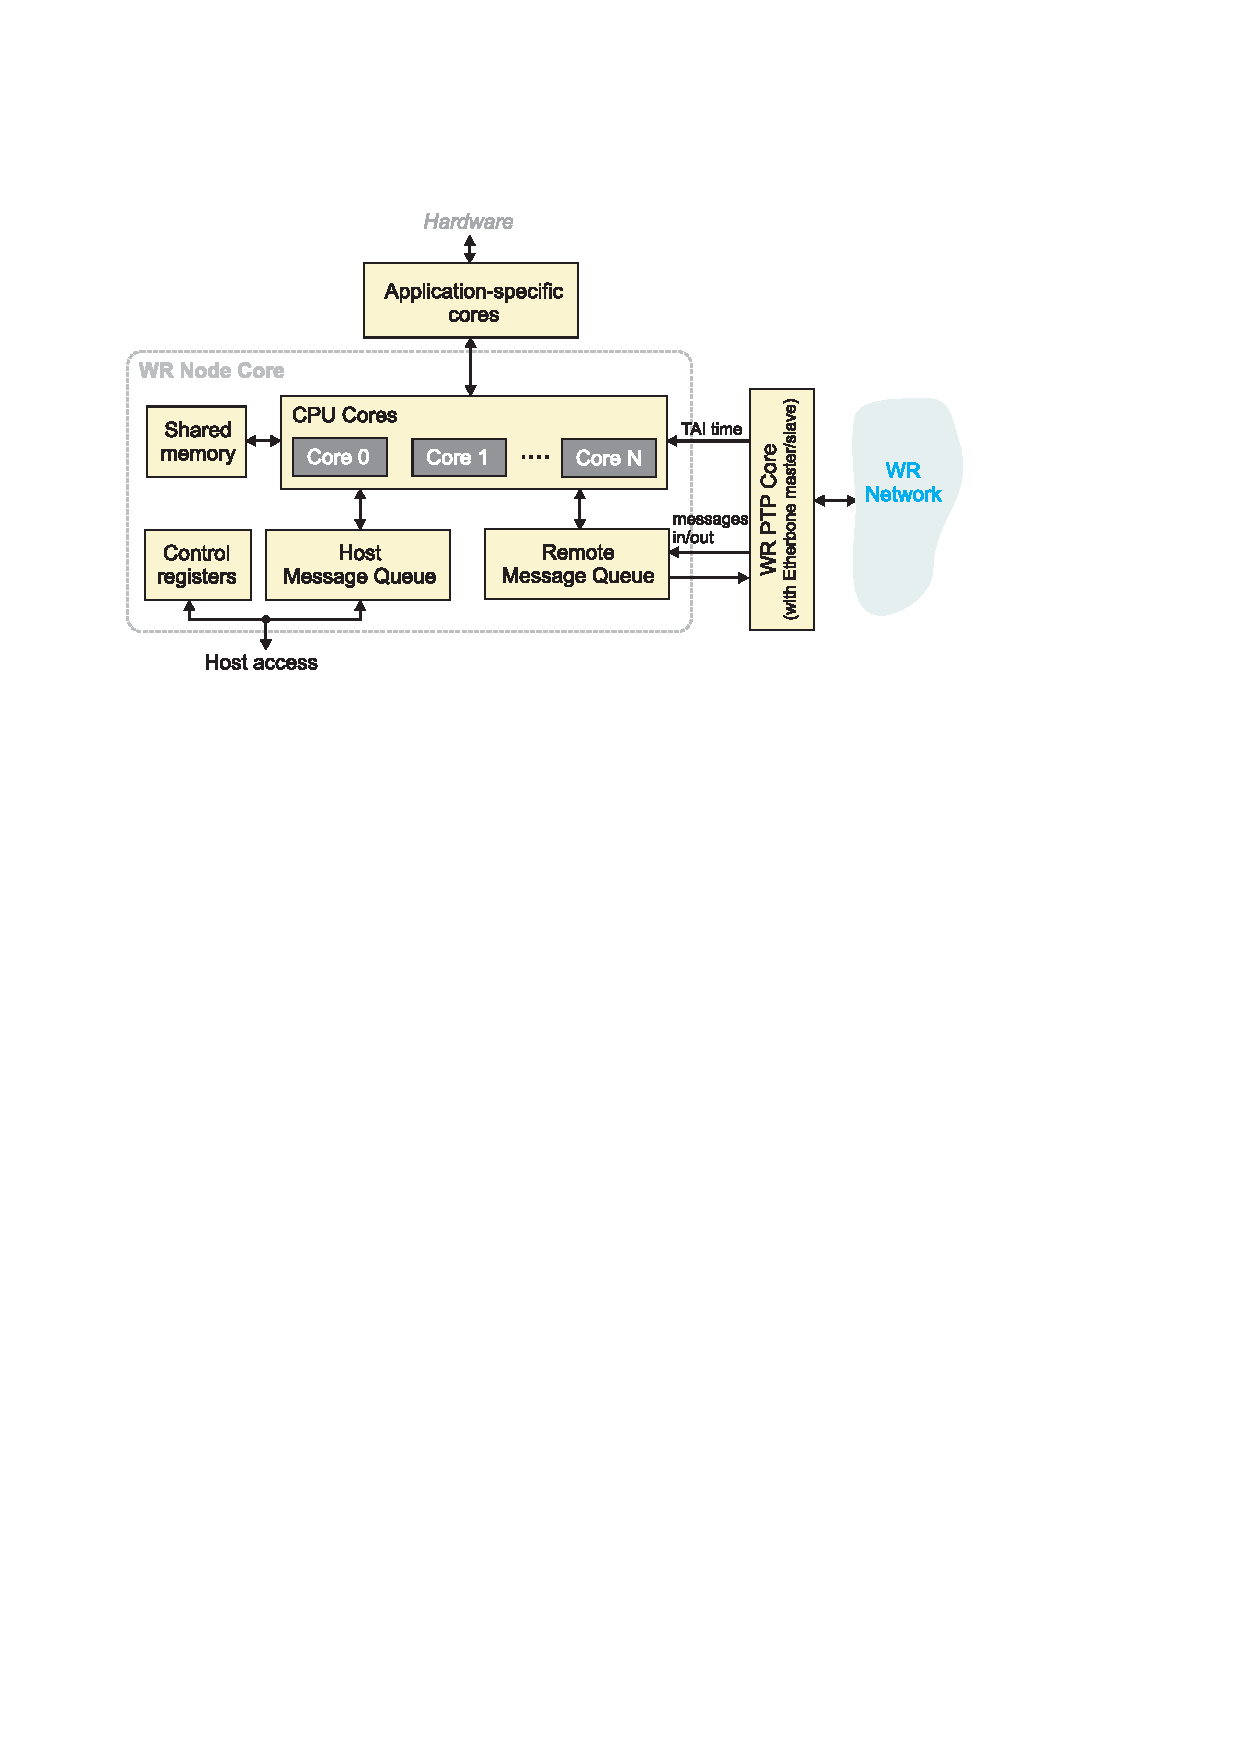
\includegraphics[width=13cm]{general.pdf}
\caption{General concept of the WR Node Core.}
\label{fig:general_concept}
\end{figure}

Figure \ref{fig:general_concept} shows a simplified block diagram of the WRNC. 
The key ingredients in the proposed design are:

\begin{enumerate}
   \item \textbf{Up to 8 CPU cores}, which:

       \begin{itemize}
       \item Execute any code the user wishes, loaded, started and stopped on request. User applications are written
         in \textit{bare metal} C (using the standard GNU tool set). Assembly may be used if necessary.
       \item Communicate between each other through a dedicated shared memory.
       \item Have no interrupts to ensure deterministic execution timing.
       \item Keep code and data in a private memory for the same reason.
       \end{itemize}
     \item \textbf{Application-specific cores and hardware.}

     The cores are accessed by the CPUs through a Wishbone bus and may
     interface with external hardware of any sort. For example, a LIST 
     node will interface with a TDC core and a Fine Delay core 
     for time tagging/producing trigger pulses. Conversely, an RF distribution node will drive a DDS 
     synthesizer and read data from a phase detector.
   \item \textbf{International Atomic Time (TAI) provided by WR.}

     The CPUs and user cores in each node in the network will have direct access to TAI, with
     a granularity of 8 nanoseconds. The system clock of the CPUs
     may be synchronous to the WR reference frequency if necessary.

   \item \textbf{Communication system}, incorporating two message queues, shared by the CPUs:
     \begin{itemize}
     \item Remote Message Queue (RMQ), which exchanges messages with remote nodes 
       in the WR network. The Etherbone protocol \cite{ebone}, developed by GSI, is used as the transport layer.
     \item Host Message Queue (HMQ), exchanging messages between the CPUs and 
       the host system. The HMQ is the primary means of communication between the 
       node and the host software (e.g. FESA \cite{fesa}). Direct access 
       to shared CPU memory or other resources may be allowed, depending on the needs of the particular application.
     \end{itemize}
\end{enumerate}
\newpage
\section{The HDL Design}

This section describes the technical details for the HDL design of the WRNC.

\subsection{Top-level}

The top level block diagram is shown in Figure \ref{fig:node_tech_block}. The WRNC talks to the external world through several interfaces:

\begin{figure}[htb]
\centering
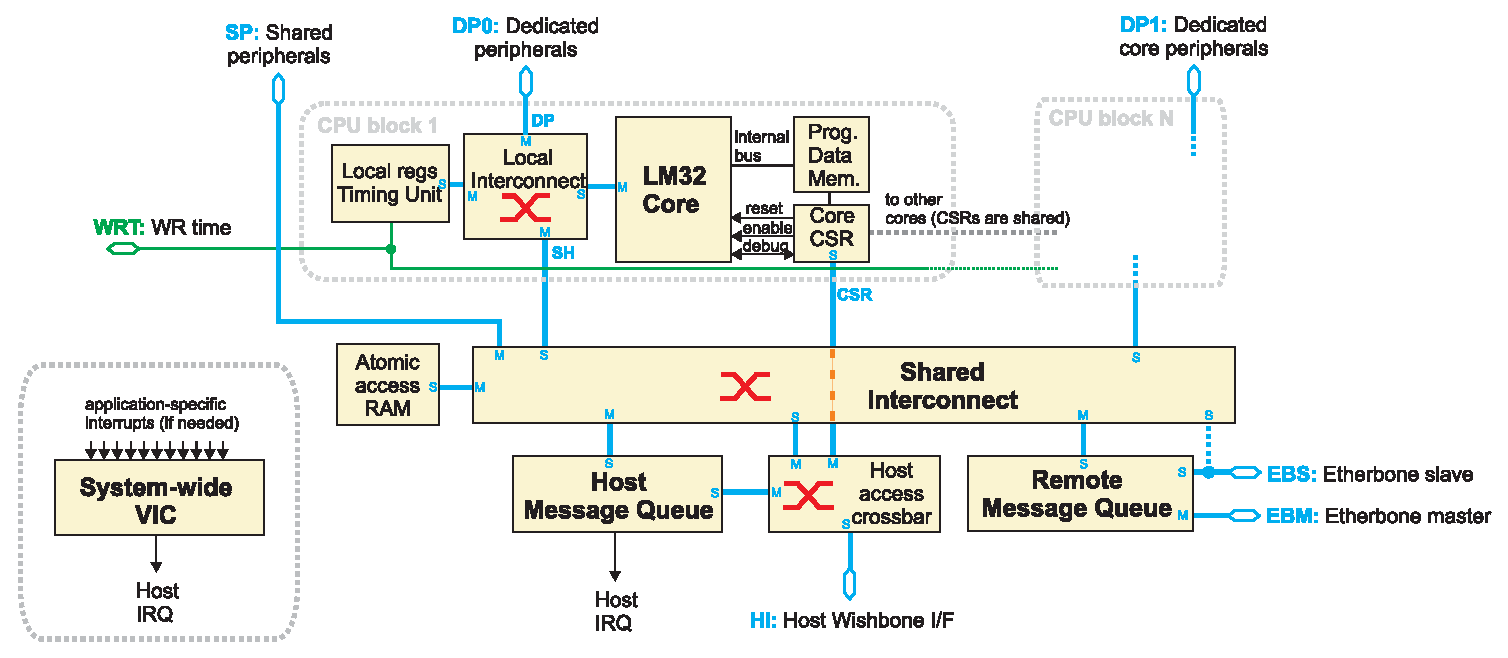
\includegraphics[width=17cm]{node_tech_block}
\caption{Structure and internal connections of the WRNC.}
\label{fig:node_tech_block}
\end{figure}


\begin{itemize}
\item \code{DPx}: A number (\code{N\_CPU}) of Wishbone masters, connecting the respective CPU cores with their private peripherals. For example, the LIST node design will have a CPU core responsible for
  reading out timestamps from a TDC Core connected to its \code{DP} port.

\item \code{SP}: shared Wishbone master, allowing all CPU cores to access certain shared peripherals. For example, an event table for the future GMT master could be stored in a large DDR memory connected through the \code{SP} port.
\item \code{HI}: shared Wishbone slave, used by the host to configure the node, access shared peripherals and Host Message Queues.
\item \code{EBM}: dedicated Wishbone master for communicating with the Etherbone master core (assembling outgoing Etherbone frames), hardwired to the RMQ.
\item \code{EBS}: dedicated Wishbone slave for receiving writes from Etherbone to the RMQ. Optionally, the \code{EBS} can be used for raw Etherbone access to the entire Shared Interconnect.


\end{itemize}


\newpage
\subsection{CPU Core Blocks}

Each node contains from one to eight (\code{N\_CPU}) CPU Core Blocks (CPU CB).  Each CPU core has its private code/data memory, a Local Registers block, a Timing Unit and a private interconnect. The CPU CB exposes the following interfaces:
\begin{itemize}
\item a Wishbone master \code{DP}, connected to the \code{DPx} port of the top level entity.
\item a Wishbone master \code{SH}, for accessing the Shared Interconnect.
\item a WR Core Timing Interface, for retrieving accurate WR time from the WR PTP Core \cite{wrpc}.
\item the Wishbone slave \code{CSR}, which allows the host to access the CPU Control Registers (CPU CSR) shared between all CPU Blocks in the node, for the purpose of firmware loading, CPU execution control and debugging.
\end{itemize}


\subsubsection{CPU Implementation}

The CPU core we have chosen is the Lattice Mico 32, a pipelined RISC CPU targeted specifically at FPGAs. The main reasons justifying the choice are:
\begin{itemize}
\item Full GCC tool set available, with a debugger.
\item Very easy to tailor to one's needs (caches/additional instructions/memory configuration).
\item Works on all major FPGA platforms.
\item Our experience (HT's and GSI's designs already use the LM32).
\end{itemize}

The LM32 implementation for the WRNC uses the following configuration:
\begin{itemize}
\item \textbf{Per-core program/data memory}.

The code and data for the program is stored in a built-in dual port RAM,
separate for each CPU core. Port 1 is reserved for the instruction pipeline, 
port 2 - for the data pipeline. There are no caches in the way to preserve 
memory access determinism. The memory size is user-configurable, up to 1 MB per CPU. 
The CPUs cannot execute code from outside this memory. Initialization of the 
CPU P/D memory is done through the CPU CSR.

\item \textbf{JTAG/Debug port:} allows real-time debugging, exposed to the host through the CPU CSR.

\item \textbf{Instruction set:} baseline LM32 + fast multiply, barrel shifter, division, fast unconditional branches, sign extension.

\item \textbf{Other features (or lack thereof):} no interrupts, no bus error handling.
\end{itemize}

All communication between the CPU core and the outside world is done through a single Wishbone master port, connected to the Local Interconnect.

\subsubsection{CPU Local Interconnect}

The Local Interconnect (CPU LI) is a non-blocking pipelined Wishbone crossbar with 1 slave and 3 master ports. The CPU uses it to communicate with:
\begin{itemize}
\item the Local Registers,
\item the Dedicated Periperhal (\code{DPx}).
\item the Message Queues, Shared Memory and Shared Peripherals through the Shared Interconnect.
\end{itemize}.

As the LI is exclusive per each CPU and has only one slave port, there are no concurrency issues when accessing the CPU's private peripherals. Duration of every access to the Local Register and DP port depends only on the Wishbone acknowledge delay of the connected peripheral.

\begin{table}[htb]
  \caption{Local Interconnect address map.}
  \centering
  \label{tab:li_addrs}
  \begin{tabular}{l p{10cm} }
    Range & Purpose \\
    \hline
    \code{0x00000 - 0xfffff} & CPU Program/Data memory \\
    \code{0x100000 - 0x1000ff} & CPU Local Registers \\
    \code{0x40000000 - 0x7fffffff} & Shared Interconnect \\
    \code{0x80000000 - 0xffffffff} & Dedicated Peripheral port\\
   \end{tabular}
\end{table}

\subsubsection{CPU Local Registers and Timing Unit}

The Local Registers (CPU LR) are the private registers of each core, providing non-arbitrated access to the most often used features of the node. The functionalities for the CPU LR are:
\begin{itemize}
\item Direct polling of the HMQ and RMQ. Since the CPUs have no interrupts, they spend most of their idle time
polling the HMQ/RMQ for newly arrived messages. If the CPUs were reading the MQ status through the Shared Interconnect, it would quickly overload (because of many WB masters accessing a single WB slave). Placing the queue slot status bits inside the LR block lets the CPUs poll as frequently as they want without disturbing the SI.
\item Providing information on the WR link and WR time status.
\item Reading current WR time (TAI seconds and 8 ns cycles).
\end{itemize}

\begin{table}[h]
  \caption{CPU LR and TU registers.}
  \centering
  \label{table:cpu_lr_regs}
  \begin{tabular}{ l l p{7cm} }
    Name & Longer name & Purpose \\
    \hline
    \code{POLL} & Polling Register & 16 bits for slot status of the HMQ and 16 bits for the slot status of the RMQ. \\
    \code{STAT} & Status Register & 1 bit for WR link status, 1 bit for WR time status. \\
    \code{TAI\_CYCLES} & TAI Time 8ns Cycles & 8 ns ticks since the beginning of the current TAI second. Reading this register latches the current TAI second in the \code{TAI\_SECONDS} register. \\
    \code{TAI\_SECONDS} & TAI Time Seconds & TAI seconds, updated on read of \code{TAI\_CYCLES}. Reading the seconds alone must be therefore preceded by a dummy read of \code{TAI\_CYCLES}. \\
    \code{TU\_CTLx} & TU Control & See Table \ref{tab:tu_ctl_reg}. \\
    \code{TU\_CNTRx} & TU Counter & Internal period counter, counting 8 ns ticks. \\
    \code{TU\_FLAGx} & TU Flag  & Set to 1 on a TU event. Clear-on-read (together with \code{TU\_HITSx}). \\
    \code{TU\_HITSx} & TU Hit counter & Increased by 1 on a TU event. Clear-on-read (together with \code{TU\_FLAGx}). \\
    \code{TU\_CYCLESx} & TU Cycles & Cycles part of the trigger time. \\
    \code{TU\_SECONDSx} & TU Seconds & Seconds part of the trigger time. \\
    \code{TU\_REPEATx} & TU Repeat Count & If the event is periodic, write the count here. \\
  \end{tabular}
\end{table}


The Timing Unit (CPU TU) lets the CPUs measure time and generate periodic events/delays. It operates by:
\begin{enumerate}
\item Waiting for a trigger condition: an offset relative to the current time, the PPS or a value of TAI.
\item Setting a clear-on-read flag in a register (since we don't have interrupts) when triggered.
\item Keeping a hit counter, counting up on each trigger event and reset on read of itself or the flag register.
\item Repeating point 2 a programmable number of times with a programmable period.
\end{enumerate}

The following conditions should be sufficient to generate accurate machine cycles split into basic periods (1.2 s, a feature commonly used in the CERN GMT Master). The TU may have multiple independent channels, depending on the implementation. 

The CPU LR and TU registers are organized as a single block with the structure described in Table \ref{table:cpu_lr_regs}.

\vskip 4mm
\textit{Note: the Timing Unit functionality and registers are subject to change.  The information above is an initial proposal for next-gen CERN timing, it's not relevant for the LIST node.} 


\begin{table}[h]
  \caption{\code{TU\_CTLx} register fields.}
  \centering
  \label{tab:tu_ctl_reg}
  \begin{tabular}{ l c p{7cm} }
    Name & Size & Purpose \\
    \hline
    \code{BUSY} & bit & 0: when the TU is not doing anything at the moment, 1: TU busy. \\
    \code{ARM} & bit & 1: to arm the TU in given \code{MODE}, 0: no action. \\
    \code{MODE} & 3 bits & Counter mode: absolute/relative/PPS. \\
    \code{CONT} & bit & 1: continuous operation, 0: repeat count defined in \code{TU\_REPEAT}. \\
    \code{STOP} & bit & 1: immediately stops the TU channel. 0: no action. \\
  \end{tabular}
\end{table}


\newpage
\subsection{Shared Control Registers}

The Shared Control Registers (CSR) expose the following functionality for the host:
\begin{itemize}
\item CPU execution control: enable/reset one or more CPUs.
\item CPU debugging: raw access to the JTAG host in each of the CPUs.
\item Program/Data memory access for firmware download.
\item Auto-enumeration/detection info for the drivers/library (TBD).
\end{itemize}

\begin{table}[htb]
  \caption{The CSR registers.}
  \centering
  \begin{tabular}{ l l p{7cm} }
    Name & Longer name & Purpose \\
    \hline
    \code{APP\_ID} & Application ID Register & User application ID for the software library to identify the node configuration \\
    \code{RESET} & CPU Reset Register & Each bit corresponds to the reset line of a CPU Core. 1 holds the CPU in reset. \\
    \code{ENABLE} & CPU Enable Register & Each bit corresponds to the enable line of a CPU Core. 1 pauses code execution. \\ 
    \code{CORE\_COUNT} & CPU Core count & Number of CPU cores in this node. \\
    \code{CORE\_SEL} & CPU Core select. & Selects the CPU core whose memory/JTAG port will be accessible through the \code{UADDR}, \code{UDATA} and \code{DEBUG} registers.\\
    \code{UADDR} & CPU Address Register. & Provides indirect access to the memory of CPU selected in the \code{CORE\_SEL} register. Write the destination address before storing/reading data through the \code{UDATA} register. \\
    \code{UDATA} & CPU Data Register. & Provides indirect access to the CPU memory. Reads/writes the memory cell pointed by \code{UADDR}. \\
    \code{DEBUG} & Debug Register. & Raw LM32 JTAG access. See Table \ref{tab:debug_register}.
  \end{tabular}
\end{table}


\begin{table}[htb]
  \caption{The \code{DEBUG} register layout.}
  \centering
  \label{tab:debug_register}
  \begin{tabular}{ l c p{7cm} }
    Name & Size & Purpose \\
    \hline
    \code{DATA} & 8 bits & LM32 Debug Unit data (read/write) \\
    \code{ADDR} & 3 bits & LM32 Debug Unit address (read/write) \\
    \code{JTCK} & bit & Writing 1 generates a JTAG TCK clock pulse. \\
    \code{JTRST} & bit & Writing 1 resets the JTAG TAP. \\
    \code{UPDATE} & bit & Writing 1 updates the JTAG address/data with the values in \code{ADDR} and \code{DATA} fields. \\
  \end{tabular}
\end{table}

\newpage
\subsection{Shared Memory}

The Shared Memory (SMEM) is a small block of RAM accessible by all CPU Cores, the Host, and Etherbone (optional). The SMEM's purpose is data/event exchange between multiple CPU cores, therefore it comes with hardware support for atomic operations:
\begin{itemize}
\item Increase/decrease (used by semaphores and queue pointers).
\item Bit set/clear/flip (used by mutexes, flags and events).
\end{itemize}

The size of SMEM is fixed to 8 kB (2048 32-bit words, no byte access), with mirroring into multiple address ranges, each responsible for a single atomic operation. The address layout is described in Table \ref{tab:smem_layout}. 

\begin{table}[h]
  \caption{Shared Memory layout.}
  \centering
  \label{tab:smem_layout}
  \begin{tabular}{ l p{9cm} }
    Address & Purpose \\
    \hline
    \code{0x0000} - \code{0x1fff} & Direct read/write access. \\
    \code{0x2000} - \code{0x3fff} & Atomic set area. On write, the corresponding memory cell is ORed with the written value. \\
    \code{0x4000} - \code{0x5fff} & Atomic clear area. On write, the corresponding memory cell is ANDed with the complement of written value.  \\
    \code{0x6000} - \code{0x7fff} & Atomic flip area. On write, the corresponding memory cell is XORed with the written value.\\
    \code{0x8000} - \code{0x9fff} & Atomic add area. On write, the corresponding memory cell is increased by the written value. Negative values are supported. \\
  \end{tabular}
\end{table}

\newpage
\subsection{Message Queues}

The Message Queues (MQs) are the heart of the WRNC's communication system, providing a simple and robust way of sending/receiving messages. The structure of the MQs is depicted in Figures \ref{fig:hmq_block} and \ref{fig:rmq_block}.

\begin{figure}[htb]
\centering
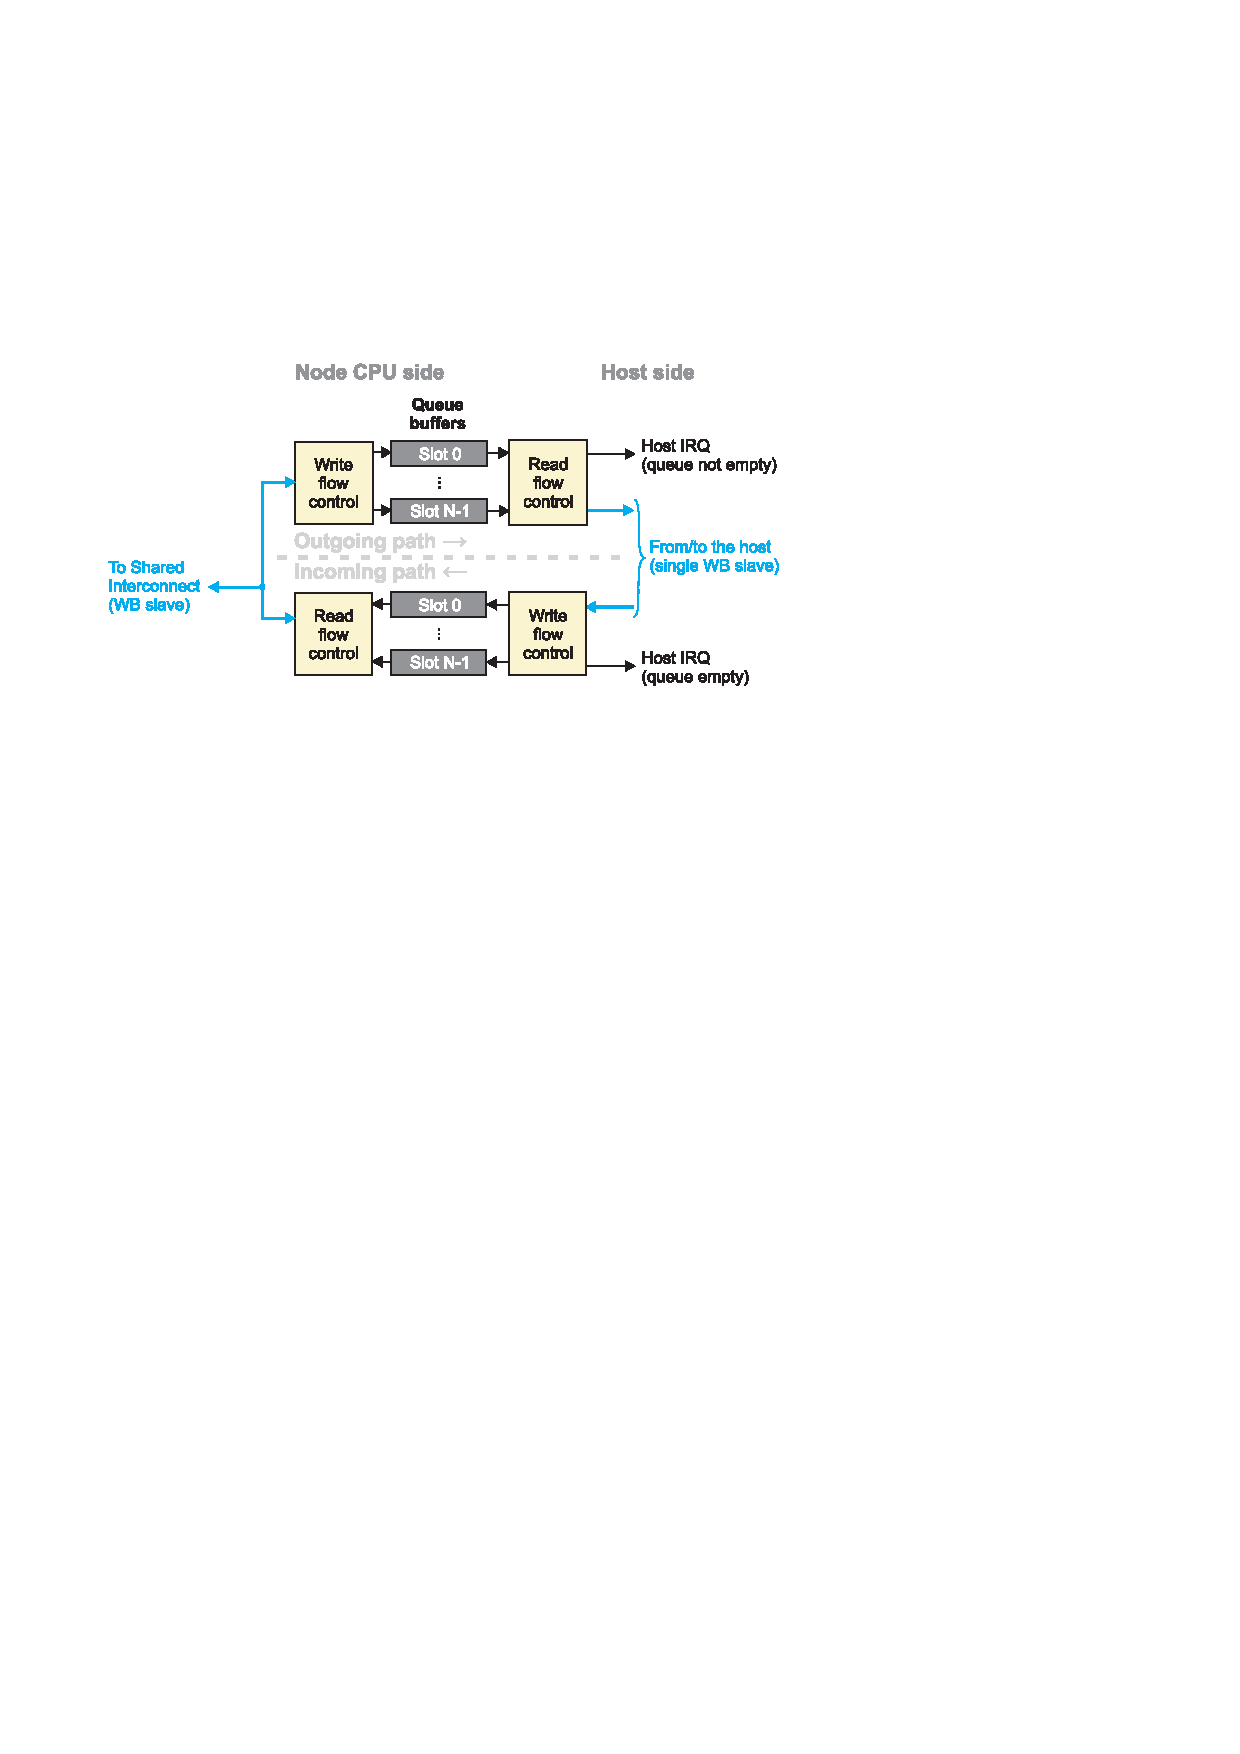
\includegraphics[width=11cm]{host_mqueue.pdf}
\caption{Block diagram of the Host Message Queue.}
\label{fig:hmq_block}
\end{figure}

\begin{figure}[htb]
\centering
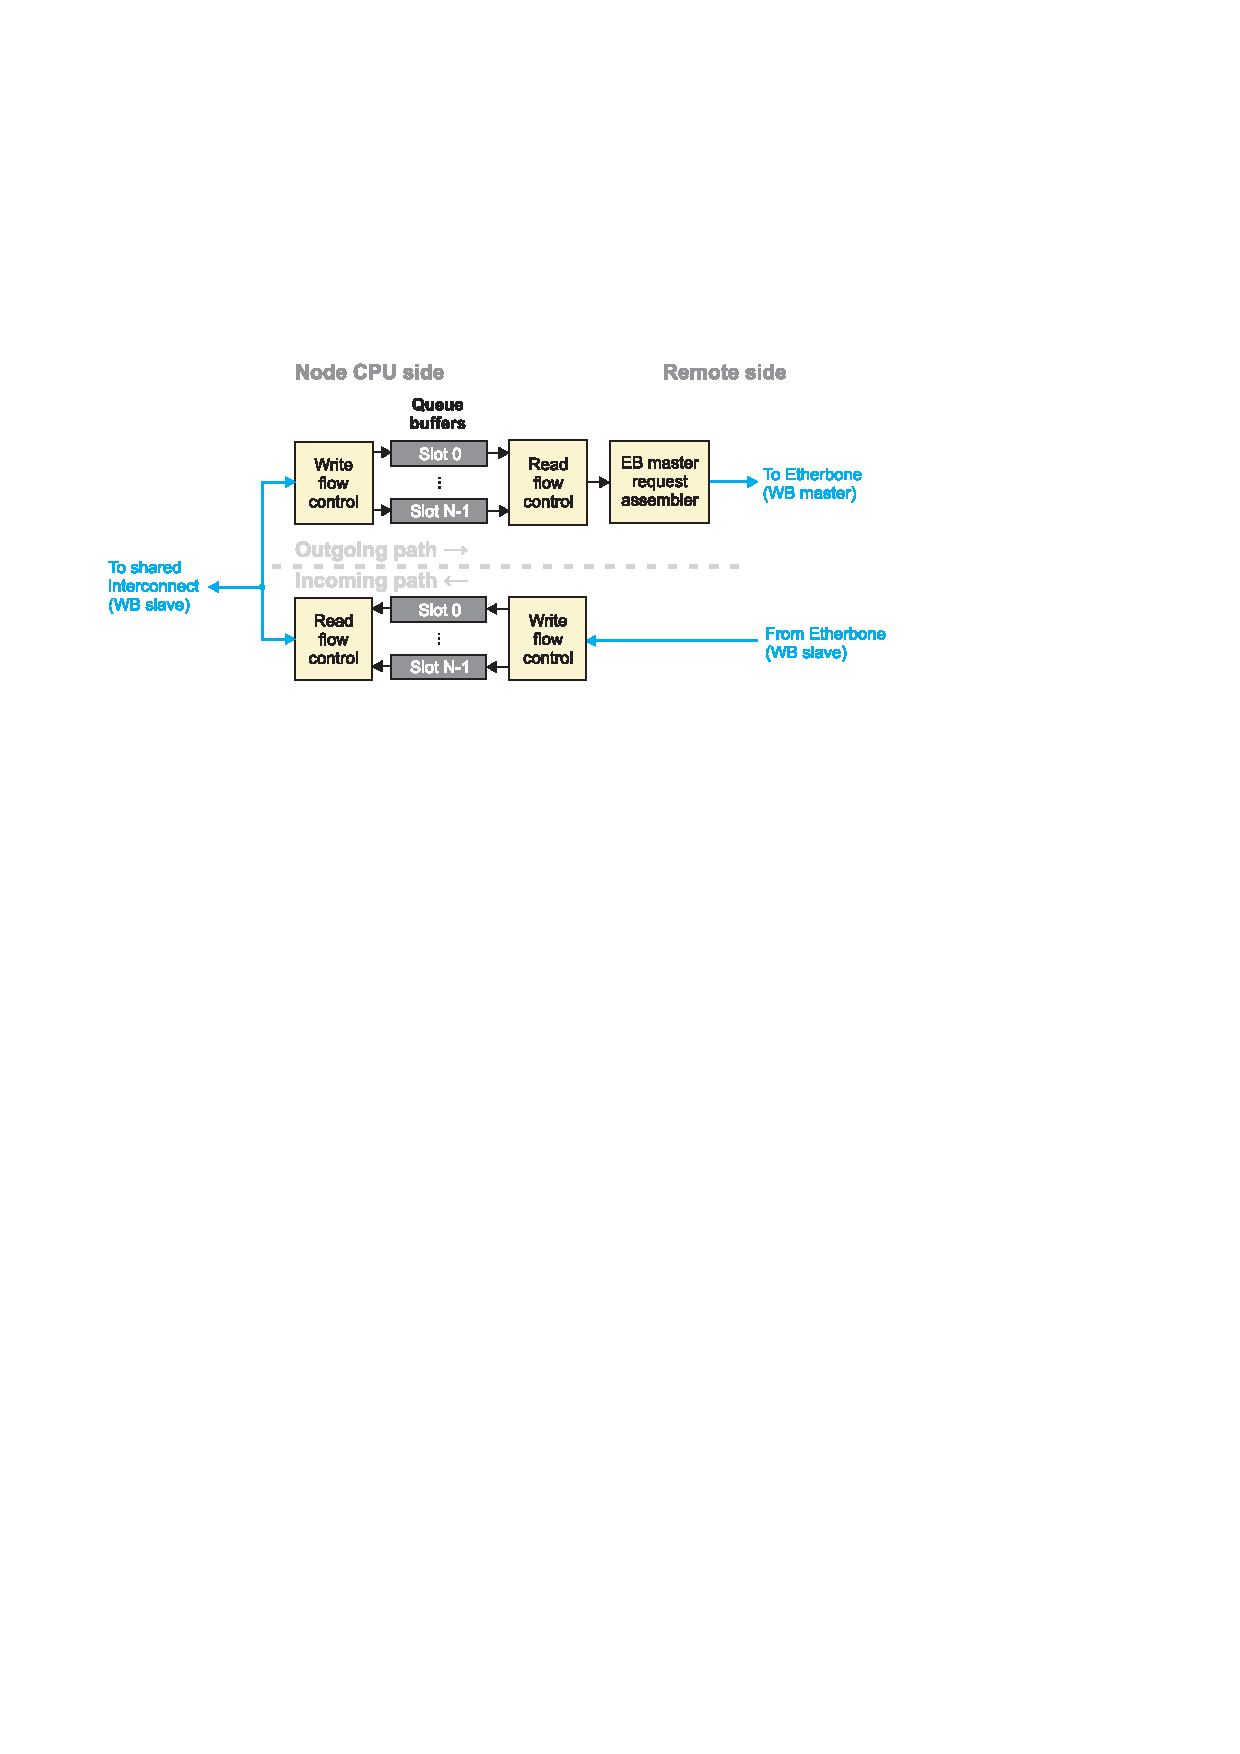
\includegraphics[width=11cm]{remote_mqueue.pdf}
\caption{Block diagram of the Remote Message Queue.}
\label{fig:rmq_block}
\end{figure}

\begin{figure}[htb]
\centering
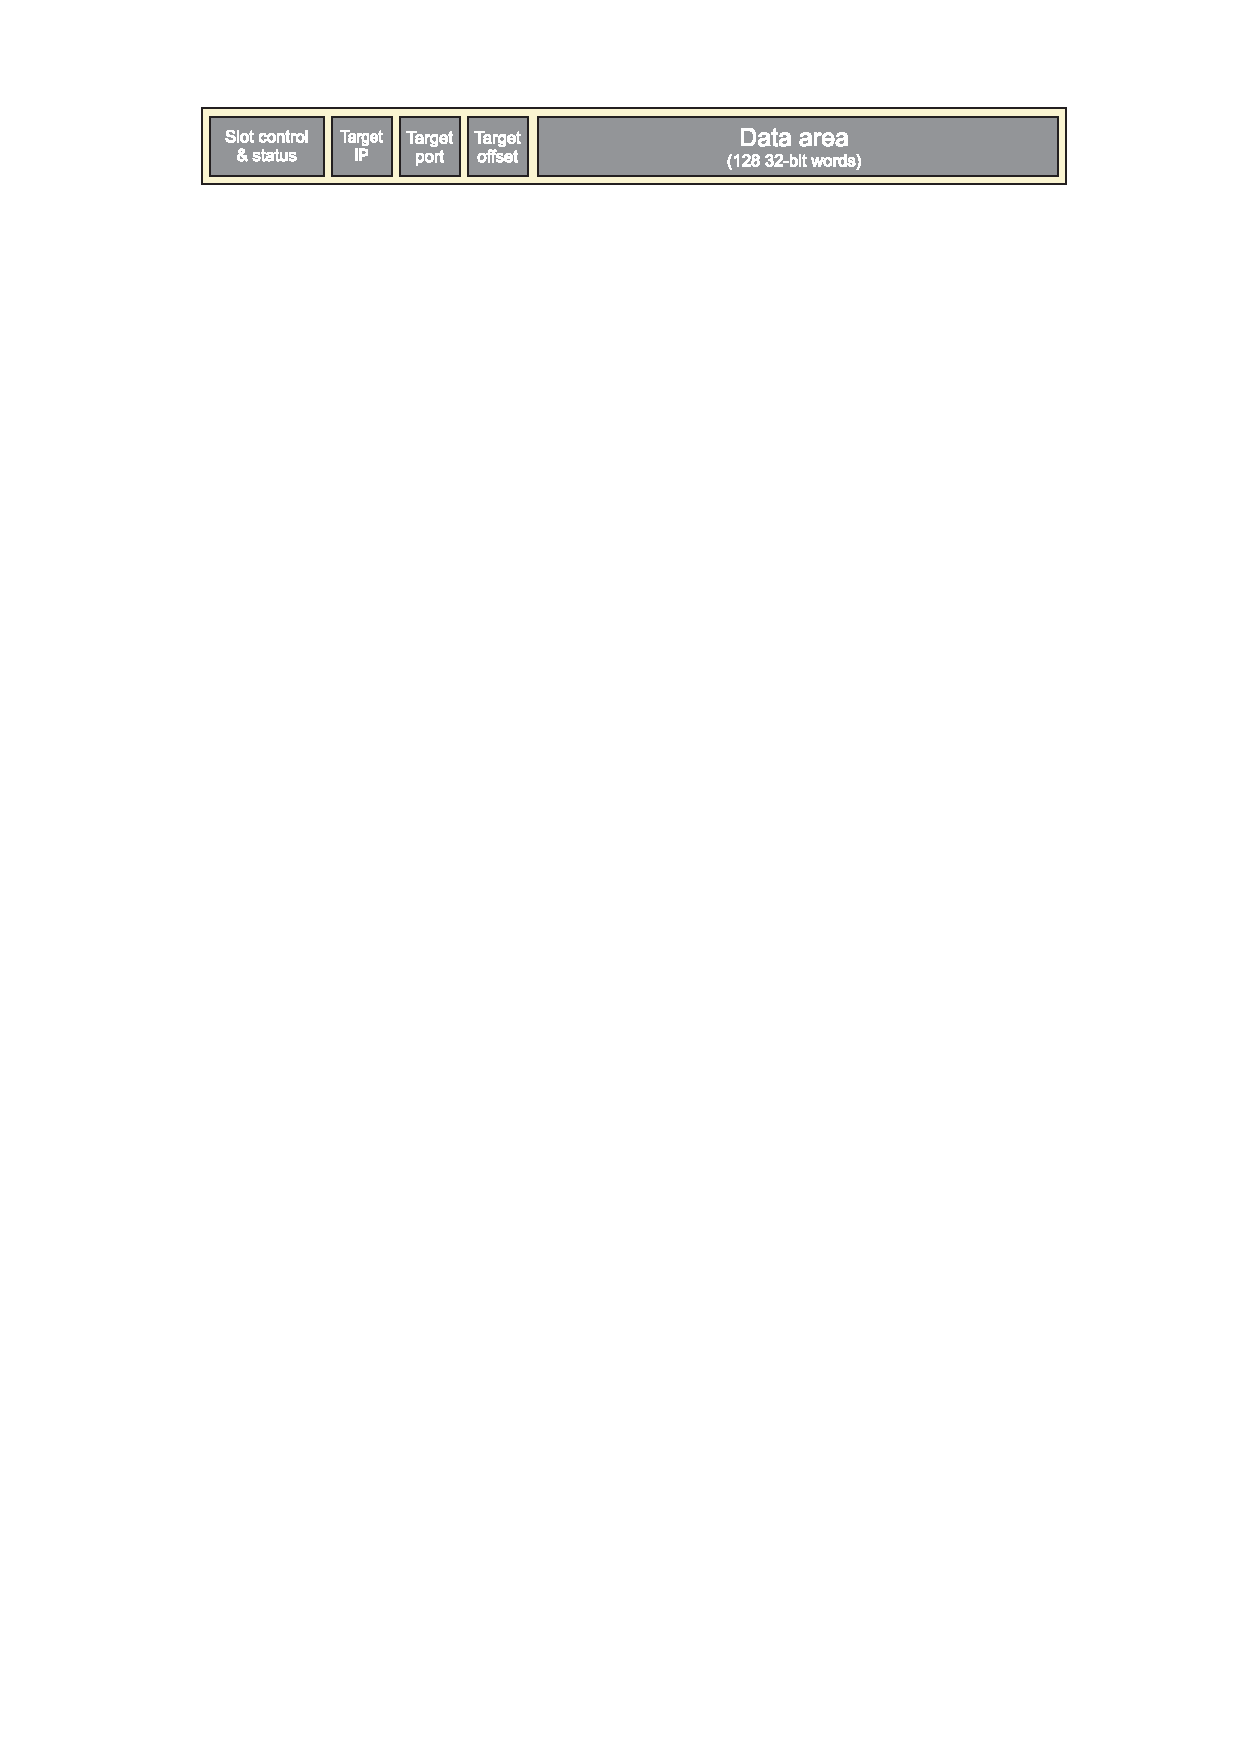
\includegraphics[width=13cm]{mqueue_slot_layout.pdf}
\caption{Layout of an MQ slot.}
\label{fig:mq_slot_layout}
\end{figure}

The principles of MQs operation are listed below:
\begin{itemize}
\item \textbf{MQs are organized as multi-word FIFOs}: The transmitter writes a number of words to an MQ outgoing slot and marks it as ready to send. The receiver side gets an indication that its MQ incoming slot is not empty, reads out its contents and indicates that it has processed the message.
\item \textbf{MQ have a number of incoming and outgoing slots}. The direction is relative to the node CPU (i.e. the node CPU receives messages from an incoming slot and sends them through an outgoing slot). Multiple slots allow handling independent message streams from independent sources. Each in/out slot consists of control/status register(s) and a payload area, allowing to transfer up to 128 32-bit words (see Figure \ref{fig:mq_slot_layout}). If the node has more than one CPU core, the CPUs must have assigned individual slots or an SMEM-based mechanism for ensuring atomic send/receive operations must be implemented. The number of slots and the size and width of each slot are configurable by a generic parameter. 
\item \textbf{Each slot can buffer multiple messages}. The depth of the slots is configurable in the VHDL entity.
\item \textbf{MQs ensure integrity} of the messages: if the message is not received completely (i.e. the Etherbone slave core reported an error), it is not received at all. Future systems using the WRNC will use an external Forward Error Correction block between the Etherbone master/slave and the WRPC to make sure no messages are dropped even in case of an error.
\item \textbf{There is no flow control}: if a MQ slot becomes full, the incoming messages are dropped. Users may implement flow control in software if needed, although in all WRNC applications currently foreseen, any buffer contention is pathological. 

\end{itemize}

\begin{figure}[htb]
\centering
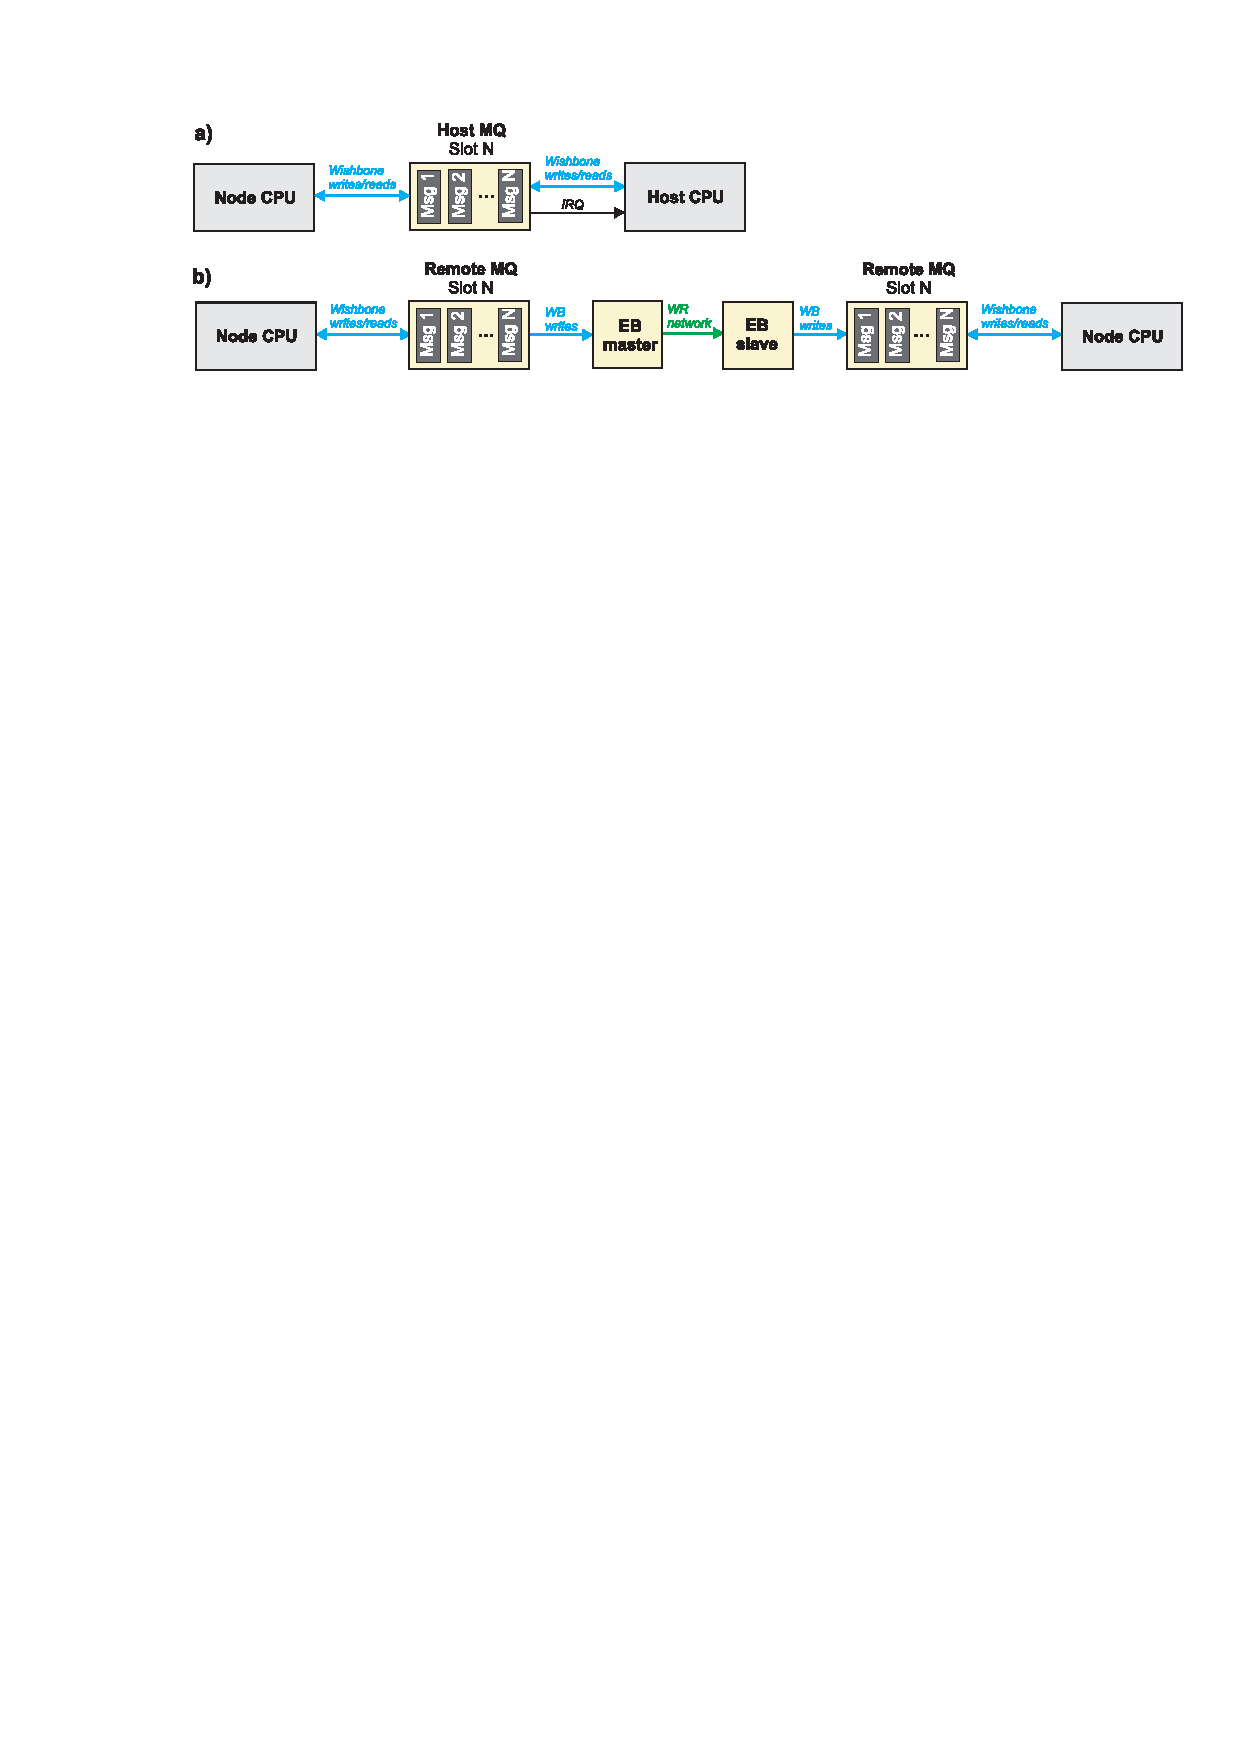
\includegraphics[width=16cm]{mqueue_msg_way.pdf}
\caption{Transmission of a message using HMQs (a) and RMQs (b).}
\label{fig:mqueue_msg_way}
\end{figure}


MQs exist in two variants:
\begin{itemize}
\item The HMQ is nothing more than a fancy FIFO between the WRN CPU Cores and the host processor. Its purpose is sending commands and exchanging data with the CPU CBs. On the host side, the empty/full status of the queue is indicated by interrupts (see Figure \ref{fig:mqueue_msg_way}a). The HMQ has two Wishbone slave ports, exposing identical register blocks to the CPU CBs and the host. A CPU writes a message to an outgoing slot in the CPU CB-side registers and the host reads it from the outgoing slot at the same address in the Host-side registers (and \textit{vice-versa} in reverse direction).

\item The RMQ casts every transmitted message into an Etherbone request, containing a sequence of write operations to MQ slot registers that will make the message appear in a given incoming slot of the RMQ in the selected remote node (see Figure \ref{fig:mqueue_msg_way}b). Message transmission using the RMQ requires setting up the IP configuration in the \code{TARGET\_} registers and initialization of the Etherbone core. The RMQ has a Wishbone slave port (for communication with the CPU CBs), a Wishbone Master port producing requests for the external Etherbone master core and a Wishbone slave port for accepting remote Etherbone traffic.
\end{itemize}

Both modules share a large part of the VHDL design and same register layout (in case of the HMQ, target IP/port/offset registers are not used).

\newpage

\begin{table}[h]
  \caption{Message Queue address map.}
  \centering
  \label{tab:mq_addr_map} 
  \begin{tabular}{l p{10cm} }
    Range & Purpose \\
    \hline
    \code{0x0000 - 0x0fff} & MQ Global Control/Status \\
    \code{0x4000 - 0x43ff} & Incoming Slot 0 (and so on)\\
    \code{0x7c00 - 0x7fff} & Incoming Slot 15\\
    \code{0x8000 - 0x83ff} & Outgoing Slot 0 (and so on)\\
    \code{0xbc00 - 0xbfff} & Outgoing Slot 15\\
   \end{tabular}
\end{table}

\begin{table}[h]
  \caption{Message Queue Global Control/Status.}
  \centering
  \label{tab:mq_global_regs} 
  \begin{tabular}{ l l p{7cm} }
    Name & Longer name & Purpose \\
    \hline
    \code{SLOT\_COUNT} & Slot Count & Number of available incoming/outgoing slots. \\
    \code{SLOT\_STATUS} & Slot Status & Each bit corresponds to one MQ slot and indicates whether it's not full (outgoing slots) and not empty (incoming slots). \\
    \code{SLOT\_IRQ\_MASK} & Slot Interrupt Mask &  Writing 1 to a particular bit enables host interrupt generation when the corresponding bit in \code{SLOT\_STATUS} is set. HMQ only. \\
    \code{SLOT\_IRQ\_COALESCE} & IRQ coalescing control & Messange count threshold and interrput timeout. Used by the driver to optimize buffer readout, exact layout TBD. \\
   \end{tabular}
\end{table}

\begin{table}[h]
  \caption{\code{COMMAND} register layout.}
  \centering
  \label{tab:mq_commands}
  \begin{tabular}{l c p{10cm} }
    Name & Size & Purpose \\
    \hline
    \code{CLAIM} & bit & Claims an incoming slot for sending a message. Issuing \code{CLAIM} on a full slot erases the oldest message making space for the new one. \\
    \code{READY} & bit & Marks the message in the slot as ready to send. When issuing a \code{READY} command, write the message size to the \code{SIZE} field.\\
    \code{DISCARD} & bit & Discards the current message. Issued after processing every incoming message. \\
    \code{PURGE} & bit & Discards all messages in the slot. \\
    \code{SIZE} & 8 bits & Size of the message to be sent (number of data words). \\
   \end{tabular}
\end{table}
\newpage

\begin{table}[htb]
  \caption{Message Queue \code{STATUS} register layout.}
  \centering
  \label{tab:mq_status_reg}
  \begin{tabular}{ l c p{7cm} }
    Name & Size & Purpose \\
    \hline
    \code{FULL} & bit & 1: the slot is full. \\
    \code{EMPTY} & bit & 1: the slot is empty. \\
    \code{COUNT} & 8 bits & number of messages in the slot. \\
    \code{SIZE} & 8 bits & number of data words in the message in the data area.\\
  \end{tabular}
\end{table}

\begin{table}[htb]
  \caption{Message Queue slot registers.}
  \centering
  \label{tab:mq_slot_regs} 
  \begin{tabular}{ l l p{7cm} }
    Name & Longer name & Purpose \\
    \hline
    \code{COMMAND} & Command register & Input commands for this message queue slots (see Table \ref{tab:mq_commands}). \\
    \code{STATUS} & Slot Status Register & Slot status (see Table \ref{tab:mq_status_reg}. \\
    \code{TARGET\_IP} & Target IP Address & IP address for the Etherbone message (RMQ only) \\
    \code{TARGET\_PORT} & Target UDP Port & UDP port for the Etherbone message (RMQ only) \\
    \code{TARGET\_OFFSET} & Target RMQ Address & Wishbone address of the target MQ slot (RMQ only) \\
    \code{DATA[0..127]} & Payload & 128 32-bit data words - payload to be sent/received. \\
   \end{tabular}
\end{table}

\newpage
\subsubsection{MQ Operations}

\begin{enumerate}
\item Transmitting a message through the HMQ (from the host or from the WRN CPU):
  \begin{itemize}
  \item Check if the required slot is available through \code{STATUS.FULL} bit.
  \item If full, keep polling the full bit or start the transmission anyway by writing a \code{CLAIM} command to the \code{COMMAND} register. Claiming a full
    slot will discard the oldest message from the queue.
  \item Write the payload.
  \item Mark the message as ready to send by issuing a \code{READY} command and indicate its size in the \code{SIZE} field of the \code{COMMAND} register. 
  \item The message TX status can be read from \code{STATUS.EMPTY} bit.
  \item Sending \code{CLAIM} before \code{READY} will clear the currently assembled message.
  \end{itemize}


\item Transmitting a message to another node through the RMQ (from the WRN CPU):
  \begin{itemize}
  \item Configure the slot's target IP, port and RMQ address. This can be done once during initialization of the node.
  \item Follow the same procedure as in point 1.
  \end {itemize}

\item Receiving a message on the WRN CPU:
  \begin{itemize}
  \item Poll the CPU CR \code{POLL} register bit corresponding to the RMQ/HMQ slot we want to receive from, until it becomes set.
  \item Process the received message.
  \item Discard it by writing \code{DISCARD} command to the slot control register.
  \end{itemize}

\item Receiving a message on the host CPU:
  \begin{itemize}
  \item Configure the interrupts.
  \item An interrupt corresponding to the chosen slot arrives: process message and discard it through \code{DISCARD} command.
  \end{itemize}
\end{enumerate}
\newpage
\subsection{Shared Interconnect}
The Shared Interconnect (SI) ensures communication between the CPU Cores, Message Queues, Shared Memory, Shared Peripherals and the host system. The SI is a full matrix, non-blocking Wishbone crossbar switch with the following arbitration policy:
\begin{itemize}
\item If multiple masters (e.g. two CPUs) talk to different slaves (e.g. CPU 0 to the the Shared Memory and CPU 2 to the HMQ), host accesses are executed concurrently.
\item If multiple masters attempt to concurrently access the same slave (e.g. two CPUs trying to send a message to the host at the very same moment), the access is arbitrated in a round-robin fashion.
\end{itemize}

\begin{table}[htb]
  \caption{Shared Interconnect address map.}
  \centering
  \label{tab:shared_intercon_addrs}
  \begin{tabular}{l p{10cm} }
    Range & Purpose \\
    \hline
    \code{0x00000 - 0x0ffff} & Shared memory \\
    \code{0x10000 - 0x1ffff} & HMQ slots (node CPU side, up to 15) \\
    \code{0x20000 - 0x2ffff} & RMQ slots (up to 15) \\
    \code{0x100000 - 0x1fffff} & Shared Peripherals port (1 MB) \\
    \code{0x40000000 - 0x7fffffff} & Shared Peripherals port (2 GB) \\
   \end{tabular}
\end{table}

\textit{Note: the SP port is mapped twice to consume less addresses in applications that have limited address space (e.g. VME).}

\subsection{Host Access Crossbar}

The Host Access Crossbar (HAC) allows the host to access the CPU CSR and the host-side registers of the HMQ without disturbing the traffic going through the CPU LIs or the SI. Host access to the SI address space is also possible (round-robin arbitrated).

\begin{table}[htb]
  \caption{Host Access Crossbar address map.}
  \centering
  \label{tab:host_xbar_addrs}
  \begin{tabular}{l p{10cm} }
    Range & Purpose \\
    \hline
    \code{0x00000 - 0x0ffff} & HMQ slots (host CPU side, up to 32) \\
    \code{0x10000 - 0x1ffff} & CPU CSR \\
    \code{0x200000 - 0x3fffff} & Shared Interconnect (small) \\
    \code{0x80000000 - 0xffffffff} & Shared Interconnect (full) \\
   \end{tabular}
\end{table}


\subsection{Interrupt support}

The WRN core itself only provides interrupts for the HMQs. If other interrupt sources are needed (for example, from the shared/dedicated peripherals), they may be connected to the common Vectored Interrupt Controller. The node driver API will provide appropriate functions for generic user space interrupt handling.

\newpage
\section{Software Interface}

The WR Node software consists of a Linux device driver and a generic user space library. User applications
are built on top of the library, there is no need for custom drivers (except for the cases which may require special
interaction with the cores connected to the WRNC).

\subsection{Device driver}

The driver is based on the \code{fmc-bus} framework, enabling the WRNC to run on any FMC carrier supported by HT's driver kit. WRN cores are automatically enumerated through Software-Defined Bus (SDB) \cite{sdb}. The driver exposes a \code{sysfs} directory for each WRN core for enumeration, initialization and debugging purposes.

Bulk communication between the driver and the user space library is implemented through a dedicated character device (one per each node) and \code{ioctl()}s. 

\subsection{Node API}

This section provides a mock-up of the WRN library C API. The API may be modified during the development of the driver.

\subsection{Initialization and node enumeration}

\begin{verbatim}
int wrn_lib_init();
void wrn_lib_exit();
\end{verbatim}
Initialization and cleanup of the WRN library.

\begin{verbatim}
int wrn_get_node_count();
\end{verbatim}
Returns the number of WR Node Cores found in the system.

\begin{verbatim}
struct wrn_dev* wrn_open_by_lun( int lun );
struct wrn_dev* wrn_open_by_fmc ( int device_id );
struct wrn_dev* wrn_open( const char *device );
\end{verbatim}
Opens the WRN with a given Logical Unit (1st case), attached to a given FMC device (2nd case) or through a direct character device path (3rd case).

\begin{verbatim}
uint32_t wrn_get_app_id( struct wrn_dev *device );
\end{verbatim}
Returns the value of the \code{APP\_ID} register of the given WRN device. May be used to 
automatically match the gateware with appropriate software built on top of the WRN library.

\begin{verbatim}
void wrn_close ( struct wrn_dev *dev );
\end{verbatim}
Closes the connection with a WRN. Note that closing doesn't cause the node core to stop working.

\subsection{CPU Control}

\begin{verbatim}
int wrn_cpu_count( struct wrn_dev* );
int wrn_cpu_stop ( struct wrn_dev*, uint32_t mask );
int wrn_cpu_start ( sturct wrn_dev *, uint32_t mask );
int wrn_cpu_reset ( sturct wrn_dev *, uint32_t mask );
int wrn_cpu_load_application ( sturct wrn_dev *, int cpu, const void *code, size_t code_size );
\end{verbatim}
Obvious functions for enumerating/starting/stopping/firmware loading for the CPUs.

\begin{verbatim}
int wrn_cpu_jtag_command ( sturct wrn_dev *, int cpu, int command, void *buffer, size_t buf_size );
\end{verbatim}
Executes a raw JTAG command on a given CPU. Foreseen for implementation of a GDB remote debugging host. The command set and arguments are TBD.

\subsection{Sending and Receiving Messages}

\begin{verbatim}
int wrn_open_slot ( sturct wrn_dev *, int slot, int flags );
void wrn_close_slot ( sturct wrn_dev *, int slot );
\end{verbatim}
Opens/closes a given HMQ slot and returns its file descriptor. The \code{flags} parameter is used
to pass the ``mode'' in which the slot will be opened:
\begin{itemize}
\item \code{WRN\_SLOT\_INCOMING} opens an incoming slot (through which we will be sending messages to the CPUs)
\item \code{WRN\_SLOT\_OUTGOING} opens an outgoing slot (through which we will be receiving messages from the CPUs)
\item \code{WRN\_SLOT\_EXCLUSIVE} opens an incoming slot without sharing its traffic to other processes which have the same slot open.
\end{itemize}
The slot can be opened with both \code{WRN\_SLOT\_OUTGOING} and \code{WRN\_SLOT\_INCOMING} flags set. In such case, the returned file descriptor is bidirectional.

\begin{verbatim}
// set of filtering rules for wrn_bind() (reverse polish notation) 
// - compare with a value (against a mask)
// - and/or/negate top of the stack

struct wrn_message_filter {

#define FILTER_OR 0
#define FILTER_AND 1
#define FILTER_COMPARE 2
#define FILTER_NOT 3

 struct rule {
   int op;           // operation 
   int word_offset;  // which word to compare
   uint32_t mask;   
   uint32_t value;
 } rules[];

 int n_rules;
};

int wrn_bind ( sturct wrn_dev *, int fd, struct wrn_message_filter *flt );
\end{verbatim}
Binds an incoming slot to receive only messages matching a given pattern. The match rule is a set of comparison and Boolean operations, written for simplicity in Reverse Polish Notation. 

\begin{verbatim}
int wrn_wait ( sturct wrn_dev *, int fd, int timeout_us );
\end{verbatim}
Waits for a message to appear in the given fd, failing if the timeout has expired (-1 to wait forever). The combination of \code{wrn\_bind()} and \code{wrn\_wait()} can be used to build powerful even filtering and polling system in an user space application.

\begin{verbatim}
int wrn_recv ( sturct wrn_dev *, int fd, void *buffer, size_t buf_size, int timeout_us );
int wrn_send ( sturct wrn_dev *, int fd, void *buffer, size_t buf_size, int timeout_us );
\end{verbatim}
Ordinary send/receive functions. Since the communication is file descriptor based, one can also
use standard POSIX functions (\code{read()}, \code{select()}, etc.) to communicate with the WRN.

\subsection{User space interrupts}

\begin{verbatim}
int wrn_enable_irq ( sturct wrn_dev *, uint32_t irq_id, int enable );
\end{verbatim}
Enables a given VIC interrupt (application-specific).

\begin{verbatim}
int wrn_wait_irq ( sturct wrn_dev *, uint32_t irq_id, int timeout_us );
\end{verbatim}
Puts the calling process to sleep until a particular interrupt has arrived. 

\subsection{Accessing Shared Memory and other peripherals}

\begin{verbatim}
#define SMEM_ATOMIC_ADD   0
#define SMEM_ATOMIC_SUB   1
#define SMEM_ATOMIC_BSET  2
#define SMEM_ATOMIC_BCLR  3
#define SMEM_ATOMIC_BFLIP 4

int wrn_smem_read ( sturct wrn_dev *, uint32_t addr, uint32_t *data);
int wrn_smem_write ( sturct wrn_dev *, uint32_t addr, uint32_t data);
int wrn_smem_op ( sturct wrn_dev *, int operation, uint32_t addr, uint32_t data);
\end{verbatim}
API for atomic operations on the Shared Memory.

\begin{verbatim}
int wrn_raw_write ( sturct wrn_dev *, uint32_t addr, uint32_t data);
int wrn_raw_read ( sturct wrn_dev *, uint32_t addr, uint32_t *data);
\end{verbatim}
Direct access to the FMC carrier's address space. Foreseen for debugging purposes. Use with caution.

\section{Application Examples}

\subsection{LIST Node}

The LIST Node HDL block diagram is shown in Figure \ref{fig:list_node_block}. The two small crossbars
between the WRNC and the FD/TDC Cores let the FD/TDC drivers access the mezzanines for initialization/management tasks. When the node CPUs are running the host never accesses these crossbars.

LIST Node configuration:

\begin{itemize}
\item CPU core 0: DP0 connected to Fine Delay FMC core (trigger output - pulse generator).
\item CPU core 1: DP1 connected to TDC FMC core (trigger input - TDC).
\item RMQ slot 0 (incoming only): received trigger messages (assigned to CPU 0).
\item RMQ slot 1 (outgoing only): transmitted trigger messages (assigned to CPU 1).
\item HMQ slot 0 (in/out): control commands for CPU 0.
\item HMQ slot 1 (in/out): control commands for CPU 1.
\item HMQ slot 2 (out only): logging channel for CPU 0 (received messages, timestamps of received, generated and missed pulses).
\item HMQ slot 3 (out only): logging channel for CPU 1 (transmitted messages and timestamps of sent pulses).
\item SMEM is not used.
\item No additional interrupts.
\item TU TAI counter used for network latency calculation and measuring task execution times.
\end {itemize}


\begin{figure}[htb]
\centering
\includegraphics[width=13cm]{node_appcase_instab.pdf}
\caption{Conceptual HDL block diagram of a LIST node.}
\label{fig:list_node_block}
\end{figure}

\subsection{Timing master}

The general idea \textit{(to be discussed)}:
\begin{itemize}
\item 2 CPU cores.
\item CPU 0, executing the timing master tasks, with context switched, non-preemptive multitasking (the LM32's processing power is very likely sufficient for directly porting the existing Timing Master assembly tasks to C without any complex rework and true parallelism).
\item CPU 1, responsible for less time-critical activities (loading event tables, etc.) and implementing the real-time functionality currently running on the MEN A20 CPU.
\item TU configured to generate 1 ms UTC-synchronized ticks that drive the task scheduler.
\item DDR memory connected to SP port, storing event tables and outgoing message log buffer.
\item RMQ slot 0 (outgoing): timing traffic.
\item HMQ slot 0 (in/out): general control.
\item HMQ slot 1 (out): log of all generated timing messages.
\item SMEM used for implementing the external conditions registers: triggering an external condition is done by atomic set/clear operations executed directly through Etherbone (bypassing the RMQ).
\end{itemize}

\subsection{Timing receiver}

The design aims to be a WR-based successor of the CTR. The current CTR design:
\begin{itemize}
\item Receives events and UTC-synchronous time base over an RS485-like link. The events are then searched against a big lookup table, which contains the configuration for the CTR's output counters that is executed if a matching event has been received. 
\item Logs received events and counter history in a large memory.
\item Forwards \textit{telegrams} (messages informing the system in advance about the machine status) to the software.
\end{itemize}

Given the granularity of current CERN timing system (1 ms time slot, up to 7 events per slot), these features can be as well implemented on a deterministic CPU. Below is a sample configuration:

\begin{itemize}
\item 1 CPU core, with DP0 connected to a CTR-like counter block. The CPU receives timing events through the RMQ slot 0, decodes them and looks up matching conditions in a locally-stored hash table. 
\item No need for a special PLL anymore, since we get the UTC/TAI timebase straight from WR.
\item DDR memory connected to SP: event/counter log buffer.
\item RMQ slot 0 (incoming): timing traffic.
\item HMQ slot 0 (in/out): general control.
\item HMQ slot 1 (out): timing events.
\item HMQ slot 2 (out): telegram readout.
\item HMQ slot 3 (out): timestamps of output pulses.
\item dedicated interrupt lines wired to the CTR counter block (counter hit indication).
\end{itemize}

\textit{Note: bidirectional WR link operation to be discussed.}

\subsection{Distributed DDS Transmitter/Receiver}

The D3S system \cite{wr-d3s} encodes an arbitrary RF frequency into UDP packets and reproduces it in any number of receiver nodes. The very brief WRN application for this project goes as follows:

\begin{itemize}
\item 1 CPU core, with DP0 connected to the DDS/phase detector core. The CPU runs the actual phase locking and data compression algorithm on baseband signal samples. Interpolation/decimation is done in dedicated HDL (part of the DDS core).
\item RMQ slot 0: incoming (receiver)/outgoing (transmitter) RF data.
\item HMQ slot 0: general purpose control.
\end{itemize}

\begin{thebibliography}{9}

\bibitem{list}
  \emph{LIST: LHC Instability Trigger Distribution System},
  CERN, 2014,
  \url{https://wikis.cern.ch/display/HT/LHC+Instability+Trigger+Distribution}
\bibitem{ebone}
  \emph{Etherbone Full specifications},
  GSI, 2013,
  \url{http://www.ohwr.org/documents/208}.
\bibitem{wrpc}
  \emph{White Rabbit PTP Core},
  CERN, 2013,
  \url{http://www.ohwr.org/documents/308}
\bibitem{fmc-bus}
  \emph{\code{fmc-bus}: an FMC abstraction layer for the Linux kernel},
  CERN, 2013,
  \url{http://www.ohwr.org/projects/fmc-bus}
\bibitem{wr-d3s}
  \emph{Distributed Direct Digital Synthesis over White Rabbit (D3S)},
  CERN, 2014,
  \url{http://www.ohwr.org/projects/wr-d3s}
\bibitem{sdb}
  \emph{Software Defined Bus specification},
  CERN, 2013,
  \url{http://www.ohwr.org/documents/256}
\bibitem{fesa}
  \emph{Frontend Software Architecture framework (FESA)},
  CERN, 2014,
  \url{http://project-fesa.web.cern.ch/project-fesa/}

\end{thebibliography}

\end{document}
